\section{include-Beziehung}

\begin{tcolorbox}[include-Beziehung]
    Die Modellierung einer \code{include}-Beziehung erlaubt das Wiederverwenden von Verhalten.\\

    \noindent
    Eine \code{include}-Beziehung dient der Ausgliederung von \textbf{redundantem Verhalten} (s.
    Abbildung~\ref{fig:usecase-include-cc}).\\

    \noindent
    Bei der Verwendung einer \code{include}-Beziehung gilt (vgl.~\cite[53]{Buh09}):


    \begin{itemize}
        \item es handelt sich um eine \textit{gerichtete} Beziehung zwischen zwei Anwendungsfällen
        \item der inkludierende Anwendungsfall fügt das Verhalten des eingefügten Anwendungsfalls in sein eigenes ein
        \item inkludieren ist \textit{nicht} optional, d.h., der inkludierte Use-Case wird immer für die Ausführung des inkludierenden Use-Cases benötigt (vgl.~\cite[65 f.]{Bal05})
        \item die Ausführung des inkludierten Use-Case ist von keiner Bedingung abhängig
    \end{itemize}

    \noindent
    Bei der \code{include}-Beziehung zeigt der Pfeil auf den einzubindenden Anwendungsfall.
\end{tcolorbox}



\begin{figure}
    \centering
    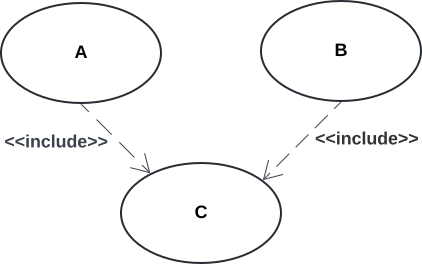
\includegraphics[scale=0.4]{part three/Anwendungsfalldiagramm/img/usecase-include}
    \caption{Notation der include-Beziehung. Die Anwendungsfälle \textbf{A} und \textbf{B} verwenden beide den Anwendungsfall \textbf{C}. (Quelle: in Anlehnung an \cite[66, Abb. 2.8-5]{Bal05})}
    \label{fig:usecase-include-cc}
\end{figure}

